\chapter{Writing the First Driver}\label{ch:first-driver}

\section{Objectives}
Communicating with real-world devices is the cornerstone of every experiment. However, devices are very different from each other. Not only is their behavior different (you can't compare a camera to an oscilloscope), but they also communicate in different ways with the computer. In this chapter,
we are going to build the first driver for communicating with a real-world device. You are going to learn about low-level communication with a serial device and, from that experience, build a reusable class that you can share with other developers.

\section{Introduction}
We can split devices into different categories depending on how they communicate with a computer. One of the most common ways to communicate is through the exchange of text messages. The idea is that the user sends a specific command, i.e., a message, and the device answers with specific information, another message. Sometimes there is no answer because it is just a command to perform an action such as an auto setting or switching off. Sometimes the message we get back contains the information we requested.

To have an idea of how commands look like, you can check the manuals of devices such as oscilloscopes or function generators. Both Tektronics\footnote{You can check the manual of an oscilloscope here: https://www.tek.com/oscilloscope/tds1000-manual} and Agilent have complete sets of instructions. If you search through their websites, you find plenty of examples. A command that you can send to a device may look like this:

\begin{minted}{text}
 *IDN?
\end{minted}

Which is asking the device to identify itself. An answer to that request would look like \texttt{Oscilloscope ID\#\#\#\#\#\#}. In this chapter, we are going to see how you can exchange messages with devices using Python.

The devices that exchange information with the computer in this way are called \textbf{message-based} devices. Some of this type of device are oscilloscopes, lasers, function generators, lock-ins, and many more. The {PFTL DAQ} device to work with this book also enters into this category. If you got the book online and not as part of a workshop, you can build your device or contact us, and we may be able to offer you one already programmed\footnote{courses@pythonforthelab.com}.

\note{There is an entire world of devices that do not communicate through messages, such as cameras, fast data acquisition cards, motorized mirrors and stages, and more. They depend on specific drivers and are harder to work with at this stage. If you are already confident programming message-based devices and need to move to non-message based ones, you can check the Advanced Python for the Lab materials.}

Remember, \textit{message-based} refers only to how the device exchanges information with the computer, and not to the actual connection between them. It is possible to connect a message-based device via RS-232, USB, GPIB, or TCP/IP. Be aware, however, that it is not a reciprocal relation: not all devices connected through RS-232 or USB are message-based. If you want to be sure, check the manual of the device and see how it is controlled. In this chapter, we are going to build a driver for a message based device.

\subsection{Scope of the Chapter}
In the introduction, we discussed that the objective is to acquire the I-V curve of a diode. You need, therefore, to set an analog output (the V) and read an analog input (the I) with the device. In this chapter, we focus
on everything we need to perform our first measurement. However, keep in mind the onion principle, which tells you that you should always be prepared to expand your code later on if the need arises.

\section{Communicating with the Device}\label{message-basedevices}
To communicate with the {PFTL DAQ}\footnote{PFTL is the shorthand notation for Python For the Lab} device, we are going to use a package called \texttt{PySerial}, which you should have already installed if you followed chapter \ref{ch:setting-up}. The first thing we can do is to list all the devices connected to the computer to identify the one in which we are interested. Plug your device via the USB port of your computer. We need to connect the {PFTL DAQ} device through the micro USB port closest to the power jack, also known as \emph{programming port}. Then, the following command in a terminal (be sure you are within the environment in which you have installed the required packages):

\begin{minted}{bash}
python -m serial.tools.list_ports
\end{minted}

\note{From now on, instead of telling you to open a terminal to run a command, if you see code which starts with a \texttt{\$} symbol, it means that you should run it in the terminal}

Depending on the operating system, the output can be slightly different. On Windows, we get something like this:

\begin{minted}{bash}
COM3
\end{minted}

While if you are on Linux you will see something like this:

\begin{minted}{bash}
/dev/ttyACM0
\end{minted}

The most important thing is to remember the number at the end. If you happen to see more than one device listed (this is very common on Mac), unplug the {PFTL DAQ}, run the command to list the ports again, note which ones appear. Plug it back and list the devices. The new one is the device in which we are interested.

Now is time to start working with the device. Start Python by running:

\begin{minted}{bash}
$ python
\end{minted}

And then we can start working directly from the command line. First, we are going to import the package we need for communication:

\begin{minted}{pycon}
>>> import serial
\end{minted}

\note{Earlier we explained that we must run in a terminal everything prepended with a \$. Lines prepended by \texttt{>>>} are lines that run in a Python interpreter. Note that there is no need to type the \texttt{>>>}}

And then we can open the communication with the device. Bear in mind that you must change the port number by the one you got earlier:

\begin{minted}{pycon}
>>> device = serial.Serial('/dev/ttyACM0') # <---- CHANGE THE PORT!
\end{minted}

Now we are ready to get started exchanging messages with the device. Before we discuss each line, let's see what you can do. The lines without \texttt{>>>} are the output generated by the code.

\begin{minted}{pycon}
>>> device.write(b'IDN\n')
4
>>> answer = device.readline()
>>> print(f'The answer is: {answer}')
The answer is: b'General DAQ Device built by Uetke. v.1.2019\n'
>>> device.close()
\end{minted}

Even if short, many things are going on in the code above. First, we import the \texttt{PySerial} package, noting that we are actually importing \texttt{serial} and not \texttt{PySerial}. Then we open the specific serial port that identifies the device. Bear in mind that serial devices can maintain only one connection at a time. If you try to run the line twice, it gives you an error letting you know that the device is busy. It happens if, for example, we try to run two programs at the same time, or if we start Python from two different terminals.

Once we established the connection, we send the \textbf{{IDN}} command to the device. There are some caveats in the process. First, the \mintinline{python}{\n} at the end, is a special character known as \texttt{newline}. It is a way to tell the device that we are
not going to send more information afterward. When a device is receiving a command, it reads the input until it knows that no more data is arriving. If we were sending a value to a device such as a wavelength, the command could look like \texttt{SET:WL:1200}. However, the device needs to know when it has received the last number. It is not the same setting the laser wavelength to $120\,\textrm{nm}$ or to $1200\,\textrm{nm}$.

The other particular detail is the \mintinline{python}{b} before the command string. Adding the \mintinline{python}{b} in front of a string is one way of telling Python to encode a string as a binary string. Devices don't understand what an \textit{A} is. The serial communication can only send a stream of 1's and 0's. Therefore, we need to transform any information we are trying to send, such as \mintinline{python}{'IDN'}, to bytes before we can send it to the device. We give a lengthier discussion about encoding strings and what it means at the end of the chapter, in section \ref{section:unicode}.

After we write to the device, we get a \texttt{4} as output. It is the number of bytes we sent, taking into account that \mintinline{python}{\n} is only one byte because it is only one character. To get the answer that the device is generating for us, we have to read from it. We use the method \mintinline{python}{readline()} for this. Then we print the answer to the screen. The answer we get also has a \texttt{\\n} and a \texttt{b}. Finally, we close the connection to the device.

We decided to use the \texttt{IDN} command because we knew it existed. But if we are starting with a new device, it is always fundamental to start by reading the manual. Manuals are our best and, perhaps, the only friend we have when developing software for controlling instruments. The {PFTL DAQ} is no exception. The manual is part of the book, and we can find it in chapter \ref{chapter:pftl-daq-manual}. It is a simple manual, but with enough information to get started, and it follows similar conventions to those we can find on more complex devices.

In the manual, the first thing we have to find is the line termination. We used the newline character because we knew it, but each device can specify something different. Some devices use the newline character as part of the commands you can send and specify that the line ending must be something else. Once we know how to terminate commands, we can go ahead and see the list of options.

Many devices (but not all) follow a standard called \href{https://en.wikipedia.org/wiki/Standard_Commands_for_Programmable_Instruments}{SCPI}. The standard makes devices easy to exchange, because the commands for all oscilloscopes are the same, for all function generators are the same, and so forth. Moreover, the SCPI standard follows a structure that makes messages easy to understand and modular. A more powerful oscilloscope, for example, has commands not available to a more basic device, but the common features are controlled by the same messages.

Now that we know how to get started with serial communication, it is time to move to more complex programs. Typing everything on the Python interpreter is not handy and takes much time. So now we can start working with files.

\subsection{Organizing Files and Folders}
When we start a new project, it is always a good idea to decide how we are going to organize the work. In the previous chapter, we have set up an environment for developing a program. That is the first step to be organized. The second step is deciding where we are going to save the files we need to write our program. The general advice is to have a folder for all the programs, for example, \texttt{Programs}. Inside, each project we work on has its folder, such as \texttt{PythonForTheLab}. Each person has their way of organizing themselves, but from now on, every time we talk about creating a file, we are referring to that base folder for the project.

\section{Basic Python Script}
The code we have developed above can also be written as a Python script, that we can run from the command line without the need to re-write everything. Create an empty file called \textbf{communicate\_with\_device.py}, and add the same code we had earlier to it:

\begin{minted}{python}
import serial

device = serial.Serial('/dev/ttyACM0')
device.write(b'IDN\n')

answer = device.readline()
print(f'The answer is: {answer}')

device.close()
\end{minted}

Now we can run the file:

\begin{minted}{bash}
$ python communicate_with_device.py
\end{minted}

\note{To be able to run the file, you need to be in the same folder where the file is. To change the folder in the terminal, you can use \texttt{cd}}

\textbf{What happens when you run the file?}

The program hangs, there is no error message and no IDN information printed to the screen. It means the program is waiting for something to let it continue. To force the stop of the program, you can press Ctrl+C, and if this does not work on Windows, you can press Ctrl+Pause/Break. Now can see the easiest way to debug when such a situation appears.

We want to know first when the program hangs, and then we can see how to fix it. So we can edit the file and add some print statements to check until which point is running:

\begin{minted}{python}
import serial
print('Imported Serial')

device = serial.Serial('/dev/ttyACM0')
print('Opened Serial')

device.write(b'IDN\n')
print('Wrote command IDN')

answer = device.readline()
print(f'The answer is: {answer}')

device.close()
print('Device closed')
\end{minted}

Rerun the script. \textbf{Where is it hanging?} Surprisingly, it is hanging during the \texttt{readline} execution. Can you understand what is going on?

There is something very different between writing on the Python interpreter and running a script: the time it takes to go from one line to the other. While you type, everything happens slowly, while when you run a script, everything happens incredibly fast. Now, the \texttt{readline} is waiting to get some information from the device, but the devices are not generating it. It means that the problem should be earlier when we sent the \texttt{IDN} message. The command is not wrong in itself, but what is happening is that between opening the communication with the device and sending the first message, we give no space.

When you establish communication with most devices, there is a small delay until you can start using it. In our case, we must add a delay between starting the communication and sending the first message. We can achieve this by doing the following:

\begin{minted}{python}
import serial
from time import sleep

device = serial.Serial('/dev/ttyACM0')
sleep(1)

device.write(b'IDN\n')
answer = device.readline()
print(f'The answer is: {answer}')
device.close()
print('Device closed')
\end{minted}

If you rerun the program, you can see that it takes a bit of time to run, but it outputs the proper message. The \texttt{sleep} function makes the program wait for a given number of seconds (also fractions) before continuing. You can try lowering the number until you get the minimum possible value. Still, in typical cases, you start the communication only once, therefore waiting 1 second or .5 seconds won't have a significant impact on the overall execution time.

\subsubsection{Reading an Analog Value}
Before we continue, it would be great to also read a value from the device, not just the serial number. If we refer again to the manual, we see that the way of getting an analog value is using the \texttt{IN} command. We can modify the code on our previous program to read a value with the device:

\begin{minted}{python}
import serial
from time import sleep

device = serial.Serial('/dev/ttyACM0')
sleep(1)

device.write(b'IDN\n')
answer = device.readline()
print(f'The answer is: {answer}')

device.write(b'IN:CH0\n')
value = device.readline()
print(f'The value is: {value}')
device.close()
print('Device closed')
\end{minted}

The value you are reading doesn't make much sense, especially if there is nothing connected to the input number 0; it is just noise. But it is an excellent first step. We can acquire a value from the real world using the device. We take care of all the things that we need to address in the following chapters.

\exercise{What happens if you use \mintinline{python}{read()} instead of \mintinline{python}{readline()}?}

\exercise{What happens if you use \texttt{read()} once, and then \texttt{readline()}?}

\exercise{What happens if you call \texttt{readline()} before writing the \texttt{IDN} command?}

\exercise{What happens if you try to write to the device after you have closed it?}


\note{\textbf{Important note about ports}: If you are using the old {RS}-232 (also simply known as \emph{serial}), the number refers to the physical number of the connection, on Windows, it is something like {COM1}, on Linux and Mac, it is something like /dev/ttyACM1. In modern computers, there are no {RS-232} connections, and most likely, we have to use a {USB} hub for them. It means that there is no physical connection
straight from the device into the motherboard. The numbering can change if we plug/unplug the cables. The {PFTL DAQ} device, since it acts as a hub for a serial connection, can show the same behavior. If you plug/unplug the device while it is being used, the port we get the second time is likely different. The second time we run the program, we need to update the information.}

\exercise{Read the manual of the {PFTL DAQ} and find a way to set an analog output to 1 Volt.}

\section{Preparing the Experiment}
Before moving forward with programming, it is time to set up the measurement we want to perform and discuss what we need to achieve it. This book revolves around the idea of measuring the I-V curve of a diode. If you are not too familiar with electronics, don't worry, it is not essential to follow the book, you can just copy the connections as shown below. If you are a bit more familiar with electronics, it is worth explaining what we are going to do.

Diodes are elements that let current flow only in one direction, but their behavior is highly non-linear. The current flowing is not proportional to the voltage applied. We chose to use an LED for the experiments because it is easy to have visual feedback on what is going on. On the other hand, we can't measure current directly. First, we need to transform it into a voltage. If you are familiar with Ohm's law, you remember the relationship:

\begin{equation}
V = I \cdot R
\end{equation}

Voltage is current times resistance. Therefore, if we want to transform a current to a voltage, we just need to add a resistance to the circuit.

To perform the experiment, we need to apply a given voltage and read a  voltage. This pattern is common to a wealth of experiments. The underlying meaning is what matters.

With the {PFTL DAQ} device, the connections that will allow us to apply a voltage and read a voltage are as follows:

\begin{figure}
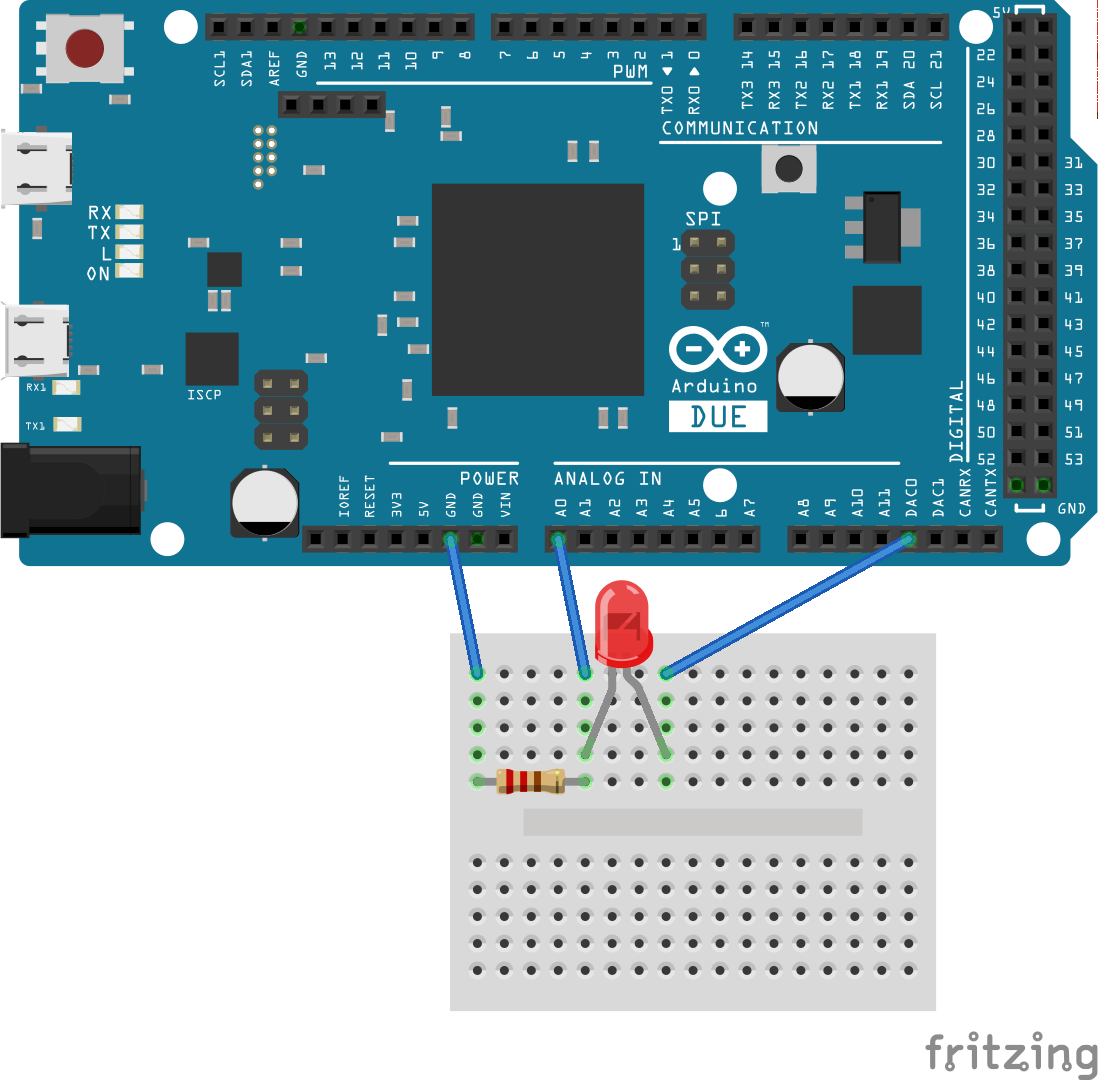
\includegraphics[width=.5\textwidth]{images/Chapter_03/IV_scheme_bb.png}
\caption{Schematic of the connections to perform the experiment}
\end{figure}

Only three cables, an LED and a resistance, are all you need to follow the rest of the book. We apply the voltage to the LED through \texttt{DAC0}. The current flows through the diode and the resistance. The voltage that we acquire at the Analog In \texttt{A0} is proportional to the current flowing through the resistance.

\exercise{Now that you have set up the experiment know how to set and read values. Acquire the I-V curve of the diode. It is a challenging exercise, aimed at showing you that it doesn't take a long time to be able to achieve an essential goal.}

\section{Going Higher Level}\label{section:going-higher-level}
We saw that communicating with a device implies taking into account parameters such as the line ending, or adding the \texttt{b} in front of messages for encoding. If the number of commands is large, it becomes very unhandy. The {PFTL DAQ} device is an exception because it is minimal, but there are still a lot of possible improvements.

If you still remember the \emph{Onion Principle} (section \ref{section:onion-principle}), it is now the time to start applying it. If you completed the last exercise, you probably have written much code to do the measurement. Perhaps you used a for loop, and acquired values in a sequence. However, if you want to change any of the parameters, you need to alter the code itself. This approach is not very sustainable for the future, especially if you are going to share the code with someone else.

Since we know how to communicate with the device, we can transform that knowledge into a reusable Python code by defining a class. Classes have the advantage of being easy to import into other projects, which are easy to document and to understand. Moreover, they are easy to expand later on. If you are not familiar with what classes are, check the appendix \ref{chapter:classes-in-python} for a quick overview. With a bit of patience and critical thinking, you can follow the rest of the chapter and understand what is going on as you keep reading.

Create a new, empty file, called \textbf{pftl\_daq.py}, and write the following into it:

\begin{minted}{python}
import serial
from time import sleep


class Device:
    def __init__(self, port):
        self.rsc = serial.Serial(port)
        sleep(1)

    def idn(self):
        self.rsc.write(b'IDN\n')
        return self.rsc.readline()

\end{minted}

The code above shows you how to start a class for communicating with a device and get its serial number. However, if you run the file, nothing happens. At the end of the file, add the following code:

\begin{minted}{python}
dev = Device('/dev/ttyACM0') #<---- Remember to change the port
serial_number = dev.idn()
print(f'The device serial number is: {serial_number}')
\end{minted}

If we rerun the code, we get the serial number of the device. Let's go line by line to understand what is going on. First, we create a class, and we define what do we want to happen when we do \texttt{Device()}. In the \texttt{\_\_init\_\_} method, we specify that the class needs a port, and we use that port to start the serial communication. The serial communication is stored as \texttt{self.rsc} in the class itself, where \texttt{rsc} is just a shorthand notation for \textit{resource}. Then we sleep for one second to give time to the communication to be established.

The second method, \texttt{idn}, just repeats what we have done earlier: we write a command, we read the line and return the output. If we look at the few lines at the bottom of the file, we now see that way of working with this class is simpler. We just use \texttt{idn()} instead of having to write and read every time.

\exercise{Once you read the serial number from the device, it does not change. Instead of just returning the value to the user, store it in the class in an attribute \mintinline{python}{self.serial_number}.}

\exercise{When you use the method \mintinline{python}{idn}, instead of writing to the device, check if the command was already used and return the value stored. This behavior is called caching, and is very useful not to overflow your devices with useless requests for data.}

\subsubsection{Reading and Setting Values}
We have just developed the most basic class, one that allows us to start the communication with the device and read its identification number. We can also write methods for reading an analog input or generating an output. The most important thing is to decide what argument each method needs. For example, reading a value only needs the channel that we want to read. Setting a value needs not only a channel but also the value itself. Also, reading a means that the method returns something. When you set an output, there is not much to return to the user.

\exercise{Write a method \mintinline{python}{get_analog_input} which takes two arguments: \mintinline{python}{self} and \mintinline{python}{channel} and which returns the value read from the specified channel.}

\exercise{Write a method \mintinline{python}{set_analog_value} which takes three  arguments: \mintinline{python}{self}, \mintinline{python}{channel} and \mintinline{python}{value} and that sets the output value to the specified port.}

Even though the exercises are important for you to start thinking by yourself, they have some caveats that are very hard to iron out if you don't have a bit of experience. First, let's look at the way of reading an analog input. We can try to develop a method that looks like this:

\begin{minted}{python}
def get_analog_input(self, channel):
    message = f'IN:CH{channel}\n'
    self.rsc.write(message)
    return self.rsc.readline()
\end{minted}

But it won't work, because even though we are adding the line ending, we are missing the \texttt{b} that we were using in the other examples. On the other hand, if we try to do something like:

\begin{minted}{python}
message = b'IN:CH{}\n'.format(channel)
\end{minted}

It will fail, because \texttt{format} only works with strings, and as soon as the \texttt{b} is added in front of a string, it is encoded to bytes. This means that we have to do it in two steps:

\begin{minted}{python}
def get_analog_input(self, channel):
    message = f'IN:CH{channel}\n'
    message = message.encode('ascii')
    self.rsc.write(message)
    return self.rsc.readline()
\end{minted}

First we form the message we want to send to the device, then we \emph{encode} it, which is the same as adding the \texttt{b} in front of a string. And then we write it to the device. After writing, we return the line with the value. We could use it as follows:

\begin{minted}{python}
dev = Device('/dev/ttyACM0') #<---- Remember to change the port
serial_number = dev.idn()
print(f'The device serial number is: {serial_number}')
volts = dev.get_analog_input(0)
print(volts)
\end{minted}

If you run the code anove, you will notice that the output still has the \texttt{b} and the \texttt{\\n}, we will work on this later. The next step is to generate an output:

\begin{minted}{python}
def set_analog_output(self, channel, output_value):
    message = f'OUT:CH{channel}:{output_value}\n'
    message = message.encode('ascii')
    self.rsc.write(message)
\end{minted}

And we can use it as follows:

\begin{minted}{python}
dev = Device('/dev/ttyACM0') #<---- Remember to change the port
serial_number = dev.idn()
print(f'The device serial number is: {serial_number}')
volts = dev.get_analog_input(0)
print(volts)
dev.set_analog_output(0, 1000)
\end{minted}

This would be all, unless we do add something extra, like reading the input after setting the output:

\begin{minted}{python}
dev = Device('/dev/ttyACM0') #<---- Remember to change the port
serial_number = dev.idn()
print(f'The device serial number is: {serial_number}')
volts = dev.get_analog_input(0)
print(volts)
dev.set_analog_output(0, 1000)
volts = dev.get_analog_input(0)
print(volts)
\end{minted}

The second time we read the analog input, we get the same value we passed to the analog output. It does not matter if it is $1000$ or $999$; it does not matter if the cables are connected or not. The value is always the same.

\exercise{Explain why when getting the analog input we get the same value that we set earlier}

This question is very tricky and requires that we read the manual of the device. In the documentation for the \texttt{OUT} command, you can see that it returns something: the same value that was passed to it. However, in our method, we are just writing to the device and not reading from it. The message waits in the queue until next time we read from it, and this happens when we try to read an analog input.

As you can see, the number of possible mistakes that we can do when developing this kind of programs is huge. On top of that, many mistakes do not generate an error, and can easily go unnoticed. When performing measurements, perhaps you don't realize the mistake on the \texttt{set\_analog\_output} until you are analyzing the data you acquired.

To solve the problem while setting the output, we just need to read from the device after setting the output:

\begin{minted}{python}
def set_analog_output(self, channel, output_value):
    message = f'OUT:CH{channel}:{output_value}\n'
    message = message.encode('ascii')
    self.rsc.write(message)
    self.rsc.readline()
\end{minted}

We are not doing anything with the information we get. We just clear it from the device.

\subsubsection{Proper Values Instead of Bytes}
To have a bit more functional class, it would be great if we could get rid of the extra \texttt{b} and \texttt{\\n} that we get every time we use the \texttt{readline()} function. First, we need to transform bytes to strings. In the previous section we transformed strings to bytes by using \texttt{.encode('ascii')}, and to no surprise, if we want to transform bytes to a string, we can do the opposite, in the \texttt{idn} method, for example:

\begin{minted}{python}
def idn(self):
    self.rsc.write(b'IDN\n')
    answer = self.rsc.readline()
    answer = answer.decode('ascii')
    return answer
\end{minted}

If you try this out, you will see that it took care of the initial \texttt{b}, but the \texttt{\\n} is still there. We need one more step to get rid of it:

\begin{minted}{python}
def idn(self):
    [...]
    answer = answer.strip()
    return answer
\end{minted}

Note that we have used \texttt{[...]} to hide the code that didn't change. Now you can go ahead and see that the output is formatted correctly.

\exercise{By using what you've learned for the \texttt{idn} method, improve the \texttt{get\_analog\_input} method so that it returns an integer. \textbf{Hint:} To transform a string to an integer, you can use \texttt{int()}, for example: \texttt{int(\'12\')}.}

\subsection{Abstracting Repetitive Patterns}
When you start to develop programs, there is a principle called \textbf{DRY}, which stands for \emph{don't repeat yourself}. Sometimes it is clear that code is repeating itself, for example, if we copy-pasted some lines. Sometimes, however, the repetition is not about code itself but a pattern. {DRY} is not a matter of just typing fewer lines of code. It is a way of reducing errors and making the code more maintainable. Imagine that after an upgrade, the device requires a different line ending. We would need to go through all your code to find out where the line ending is used and change it. If we would specify the line ending in only one location, changing it would require just to change one line.

First, we can specify the default parameters for our device. They will be all the constants that we need in order to communicate with it, such as line endings. We can define them just before the \mintinline{python}{__init__} method, like this:

\begin{minted}{python}
class Device:
    DEFAULTS = {'write_termination': '\n',
                'read_termination': '\n',
                'encoding': 'ascii',
                'baudrate': 9600,
                'read_timeout': 1,
                'write_timeout': 1,
                }
    def __init__(self, port):
        [...]
\end{minted}

You can see that there is much new information in the class. We have established a clear place where both the read and write line endings are specified (in principle they don't need to be the same), we also specify that we want to use ascii to encode the strings and that the baud rate is 9600. This value is the default of PySerial, but it is worth making it explicit in case newer devices need a different option. We also specify timeouts, which are allowed by PySerial and would prevent the program from freezing if writing or reading takes too long.

It is normally good practice to separate the instantiation of the class with the initialization of the communication. One thing is creating an object in Python, and the other is to establish communication with a real device. Therefore, we can rewrite the class like this:

\begin{minted}{python}
def __init__(self, port):
    self.port = port
    self.rsc = None

def initialize(self):
    self.rsc = serial.Serial(port=self.port,
                        baudrate=self.DEFAULTS['baudrate'],
                        timeout=self.DEFAULTS['read_timeout'],
                        write_timeout=self.DEFAULTS['write_timeout'])
    sleep(1)
\end{minted}

You can see that there are some major changes to the code, but the arguments of the \mintinline{python}{__init__} method are the same. In this way, code already written does not fail if we change the number of arguments of a method. When we do this kind of change, it is called \emph{refactoring}. It is a complex topic, but one of the best strategies you can adopt is not to change the number of arguments functions take, and the output should remain the same. In the class, the \mintinline{python}{__init__} definition looks the same, but its behavior is different. Now, it just stores the \mintinline{python}{port} as the attribute \mintinline{python}{self.port}. Therefore, to start the communication with the device, we need to do \mintinline{python}{dev.initialize()}. You can also see that we have used almost all the settings from the \mintinline{python}{DEFAULTS} dictionary to start the serial communication.

After we do these changes, we should also update the code we use to test the device:

\begin{minted}{python}
dev = Device('/dev/ttyACM0') #<---- Remember to change the port
dev.initialize()
serial_number = dev.idn()
print(f'The device serial number is: {serial_number}')
volts = dev.get_analog_input(0)
print(volts)
dev.set_analog_output(0, 1000)
volts = dev.get_analog_input(0)
print(volts)
\end{minted}

So far the only difference with the previous code is the \mintinline{python}{__init__} method. We have to improve the rest of the class. We already know that for message-based devices there are two operations: \textbf{read} and \textbf{write}. However, we will only read after a write (remember, we should ask something from the device first.) It is possible to update the methods of the class to reflect this behavior. Since all the commands of the device return a value, we can develop a method called \texttt{query}:

\begin{minted}{python}
def query(self, message):
    message = message + self.DEFAULTS['write_termination']
    message = message.encode(self.DEFAULTS['encoding'])
    self.rsc.write(message)
    ans = self.rsc.readline()
    ans = ans.decode(self.DEFAULTS['encoding']).strip()
    return ans
\end{minted}

In this way, we take the message, append the proper termination, and encodes it as specified in the \texttt{DEFAULTS}. Then, it writes the message to the
device exactly as we did before. Then we read the line, we decode it using the defaults and strip the line ending. Now it is time to update the other methods of the class to use the \texttt{query} method we have just developed. Let's start with \texttt{idn}, which now looks like this:

\begin{minted}{python}
def idn(self):
    return self.query('IDN')
\end{minted}

And the same we can do for the other methods:

\begin{minted}{python}
def get_analog_input(self, channel):
    message = 'IN:CH{}'.format(channel)
    ans = self.query(message)
    ans = int(ans)
    return ans

def set_analog_output(self, channel, output_value):
    message = 'OUT:CH{}:{}'.format(channel, output_value)
    self.query(message)
\end{minted}

For such a simple device, perhaps the advantages of abstracting patterns are not evident. It is something that happens very often in more extensive programs, and being able to identify those patterns can make the difference between a successful program and something only one person can understand. Note that even if we have changed the methods for identifying, reading, and setting analog values, there is no need to update the example code.

It is important to see that we achieved the communication with the device through the resource \mintinline{python}{self.rsc} that is created with the method \mintinline{python}{initialize}. There is a common pitfall with this command. If we try to interact with the device before we initialize it, we get an error like the following:

\begin{minted}{python}
AttributeError: 'NoneType' object has no attribute 'write'
\end{minted}

We now remember why this happened, but it is very likely that in the future, either we forget or someone else is using our code, and the error message that appears is incredibly cryptical. Therefore, we suggest you do the following:

\exercise{Improve the \texttt{query} method to check whether the communication with the device has initialized. If it hasn't, you can print a message to the screen and prevent the rest of the program from running.}

When we develop code, we must always keep an eye on two people: the future us and other users. It may seem obvious now that we initialize the communication before attempting anything with the device, but in a month, or a year, when we dig up the code and try to do something new, we are going to be another person. We won't have the same ideas in our mind as right now. Adding safeguards are, on the one hand, a great way of preserving the integrity of your equipment; on the other, it cuts down the time it takes to find out what the error was.

There is only one last thing that we are missing. We have completely forgotten to add a proper way of closing the communication with the device. We can call that method \texttt{finalize}:

\begin{minted}{python}
def finalize(self):
    if self.rsc is not None:
        self.rsc.close()
\end{minted}

We first check that we have actually created the communication by verifying that the \mintinline{python}{rsc} is not \mintinline{python}{None}. Then, we can update our example code at the bottom of the file to actually use the finalize method:

\begin{minted}{python}
dev = Device('/dev/ttyACM0') #<---- Remember to change the port
dev.initialize()
serial_number = dev.idn()
print(f'The device serial number is: {serial_number}')
volts = dev.get_analog_input(0)
print(volts)
dev.set_analog_output(0, 1000)
volts = dev.get_analog_input(0)
print(volts)
dev.finalize()
\end{minted}

We may wonder why things work out fine even though we didn't have the \texttt{finalize} method in place. The answer is that PySerial is smart enough to close the communication with the device when it realizes we will no longer use it. However, it is not always the case if the program crashes. Sometimes the communication stays open, and the only way to regain control of the device is by manually shutting it off and on again. If this happens, we must always check whether the port changed.

\section{Doing something in the \emph{Real World}}
Until now, everything looked like a big exercise of programming but now it is time to start interacting with the real world. As we know from reading the manual, the {PFTL DAQ} device can generate analog outputs, and the values we can use go from $0$ to $4095$. We can expand slightly the code below the class in order to make the LED blink for a given number of times, and report the measured voltage when it is either on or off:

\begin{minted}{python}
dev = Device('/dev/ttyACM0') #<---- Remember to change the port
dev.initialize()
serial_number = dev.idn()
print(f'The device serial number is: {serial_number}')
for i in range(10):
    dev.set_analog_output(0, 4000)
    volts = dev.get_analog_input(0)
    print(f'Measured {volts}')
    sleep(.5)
    dev.set_analog_output(0, 0)
    volts = dev.get_analog_input(0)
    print(f'Measured {volts}')
    sleep(.5)
\end{minted}

With this simple code, we can switch on and off the LED 10 times, and we print to screen the values that we are reading when it is on or off. There are two things to note: first, we are switching it ON by using a value of $4000$. We have selected it because it is high enough to switch the LED on, but it has no units, it is not a voltage. The same with the value reported by the \texttt{get\_anlog\_input}, which is just an integer, but we have no idea, yet, of what it means.

Before we can proceed, we must understand how to transform Analog signals to digital values and the opposite.

\subsection{Analog to Digital, Digital to Analog}\label{subsection:digitazing}
Almost every device that we find in the lab transforms a continuous signal to a value that can be understood by the computer. The first step is to transform the quantity you are interested in a voltage. Then, we need to transform the voltage (an analog signal) to something with which the computer can work. Going from the real world to the computer space is normally called \emph{digitizing} a signal. The main limitation of this step is that the space of possible values is limited, and therefore we have discrete steps in our data.

For example, the {PFTL DAQ} device establishes that when reading a value, it uses 10 bits to digitize the range of values between $0\,\textrm{V}$ and $3.3\,\textrm{V}$. In the real world, the voltage is a real number that can take any value between $0\,\textrm{V}$ and $3.3\,\textrm{V}$. In the digital world, the values are going to be integers between $0$ and $1023$ ($2^{10}-1$). It means that if the device gives us a value of $0$, we can transform it to $0\,\textrm{V}$. A value of $1023$ corresponds to $3.3\,\textrm{V}$, and there is a linear relationship with the values in between.

\begin{center}
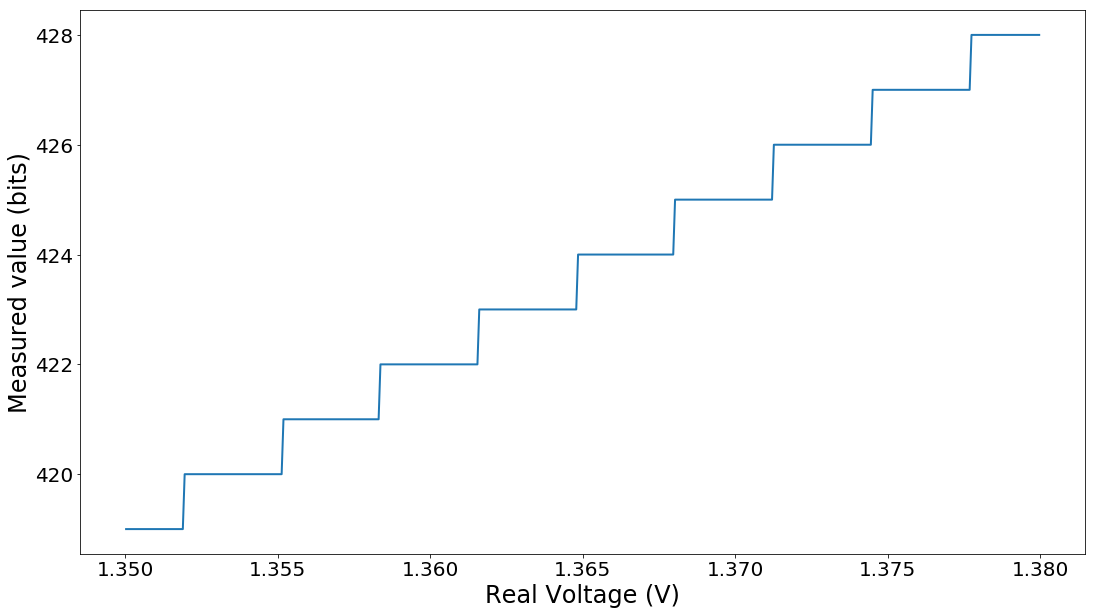
\includegraphics[width=.6\textwidth]{images/Chapter_03/digitalization.png}
\end{center}

The figure above shows a detail of how the digitalization looks like for a range of voltages. You see the discrete steps that the digital value takes for different voltages. Digitizing signals is a critical topic for anybody working in the lab. There is a whole set of ramifications regarding visualization, data storage, and more.

Particularly, the {PFTL DAQ} has a different behavior for reading than for setting values. The output channels take $4095$ ($2^{12}-1$) different values, i.e. they work with 12 bits instead of 10. Knowing the number of bits, also allows us to calculate the minimum difference between two output values:

\begin{equation}
 \frac{3.3\,\textrm{V} - 0\,\textrm{V}}{4096} \approx 0.0008\,\textrm{V} = 0.8\,\textrm{mV}
\end{equation}

The equation above shows how the resolution of the experiment is affected by the digitalization of the signals. We can't create voltages with a difference between them below $0.8\,\textrm{mV}$, and we are not able to detect changes below $3\,\textrm{mV}$. Later in the book, we come back to this discussion when we need to decide some parameters for visualizing our data.

Digitizing is everywhere. Digital cameras have a certain \emph{bit depth}, which tells us which range of values they can cover or, in other words, their dynamic range. Oscilloscopes, function generators, acquisition cards, they all have a precise digital resolution. When planning experiments, we always need to keep an eye on these values to understand if the devices are appropriate for the measurement we want to perform.

\exercise{We have used a for-loop to switch on and off the LED, and we have also displayed the voltage measured, but without units. Update the code so that instead of printing integers it prints the read value in volts.}

\section{Doing an experiment}
At this stage, we can easily communicate with the device; we can set an output and measure a voltage. It means that we have developed everything that we needed to measure the current that goes through the LED. We only need to combine setting an analog output and then reading an analog input. Since we are going to develop this with a more consistent approach, we leave it as an exercise:

\exercise{Write a method that allows you to linearly increase an analog output in a given range of values for a given step. \textbf{Hint:} the function \texttt{range} allows you to do this: \texttt{range(start, stop, step}. If you use this method, you should be able to see the LED switching gradually on.}

\exercise{Improve the method so that we can read analog values and store them once the measurement is complete. Returning the values can be a good idea so that we can use them outside of the object itself.}

\exercise{If you already have some experience with Python, you can also make a plot of the results. We cover this topic, later on, so don't stress too much about it now.}

If you tried to solve the exercises, you probably noticed that by having classes, our code is straightforward to use. It would be simple to share it with a colleague that has the same device, and they can adapt and expand it according to their needs. We should also keep in mind that when working with devices, it may very well be that someone else has already developed a Python driver for it, and we can just use it. One of the keys to developing sustainable code is to compartmentalize different aspects of it. Don't mix the logic of a particular experiment with the capabilities of a device, for example, is precisely the topic of the following chapter.

\textbf{Remember the Onion}: We have discussed in the Introduction, that we should always remember the onion principle when developing software. If we see the outcome of these last few exercises, we notice that we are failing to follow the principle. We have added much functionality to the driver class that does not reflect what the device itself can do. The {PFTL DAQ} doesn't have a way of linearly increasing an output, and we have achieved that new behavior with a loop in a program. Therefore, the proper way of adding extra functionality would be by adding another layer to the program, as we see in the next chapter.

Before moving forward, it is also important to discuss other libraries that may come in handy. We are not the first ones who try to develop a driver for a device. The pattern of writing and reading, initializing, and many more that we haven't covered, were faced by many developers before ourselves. It means that there are libraries already available that can speed up a lot the development of drivers. Let's see some of them.

\section{Using PyVISA}\label{section:pyvisa}
Some decades ago, prominent manufacturers of measurement instruments sat together and developed a standard called \href{https://en.wikipedia.org/wiki/Virtual_instrument_software_architecture}{Virtual instrument software architecture}, or VISA for short. This standard allows communicating with devices independently from the communication channel selected, and from the backend chosen. Different companies have developed different backends, such as NI-VISA, or TekVISA, but they \emph{should} be interchangeable. The backends are generally hard to install and do not work on every operating system. But they do allow to switch from a device connected via Serial to a device connected via USB or GPIB without changing the code.

To work with VISA instruments, we can use a library available for Python called \texttt{pyvisa}. There is also a pure Python implementation of the VISA backend called \mintinline{python}{pyvisa-py}, which is relatively stable even if it is still work in progress. It does not cover 100\% of the VISA standard, but for simple devices like the {PFTL DAQ} it should be more than enough. For complex projects, the solutions provided by vendors such as Tektronix or National Instruments may be more appropriate. In the next few paragraphs, we see how to get started with pyvisa-py, but it is not a requirement of the book. We decided to show it here to have it as a reference for other projects.

First, we need to install \mintinline{python}{pyvisa}, which is a wrapper around the VISA standard. Either with pip:

\begin{minted}{bash}
 pip install pyvisa
\end{minted}

Or with conda:

\begin{minted}{bash}
 conda install -c conda-forge pyvisa
\end{minted}

In case we don't have a VISA backend on our computer, we need to install one, and the easiest is the python implementation:

\begin{minted}{bash}
 pip install pyvisa-py
\end{minted}

or with conda:

\begin{minted}{bash}
 conda install -c conda-forge pyvisa-py
\end{minted}

There is also an interesting dependency missing: PySerial. Neither Pyvisa nor Pyvisa-py depend on PySerial. If we are going to communicate with serial devices, we should install that package ourselves (and the same is true for USB, GPIB, or any other communication standard.) The documentation of pyvisa-py\footnote{https://pyvisa-py.readthedocs.io} has handy information.

To quickly see how to work with PyVISA, we can start in a python interpreter, before going to more complex code. VISA allows you to list your devices:

\begin{minted}{pycon}
 >>> import visa
 >>> rm = visa.ResourceManager('@py')
 >>> rm.list_resources()
 ('ASRL/dev/ttyACM0::INSTR',)
 >>> dev = rm.open_resource('ASRL/dev/ttyACM0::INSTR')
 >>> dev.query('IDN')
 'General DAQ Device built by Uetke. v.1.2017\n'
\end{minted}

We make explicit the backend we want to use by calling \texttt{ResourceManger}. In some cases, visa can automatically identify the backend on the computer. Then, we list all the devices connected to the computer. Bear in mind that this depends on the other packages that we installed. For example, we have only PySerial, and therefore pyvisa-py only lists serial devices. We can install PyUSB to work with USB devices, or GPIB, and so forth. The rest of the code is very similar to what we have done before. It becomes clear why we decided to call \emph{resource} the communication with the device.

Pay attention to the \texttt{query} method that we use to get the serial number from the device. We didn't develop it. PyVISA already took care of defining query for us. Not only PyVISA takes care of the query method, but they have plenty of options that we can use, such as transforming the output according to some rules or establishing the write termination. If we were to follow the pyVISA path, we could start by reading their documentation\footnote{https://pyvisa.readthedocs.io}.

\textbf{Why didn't we start with pyVISA?}. There are several reasons. One is pedagogical. It is better to start with as few dependencies as possible, so we can understand what is going on. We had to understand not only what commands are available, but we also had to be aware of the encoding and line termination. We made explicit the fact that to read from a device, we first have to write something to it. Once you gain confidence with the topics covered in this chapter, you can explore other solutions and alternatives. PyVISA is only the tip of the iceberg.

\section{Introducing Lantz}\label{section:lantz}
Defining a class for your device was a massive step in terms of usability. You can easily share your code with your colleagues, and they can immediately start using what you have developed with really few extra lines of code. However, there are many features that we may want but that someone needs to develop. For example, imagine that we want to limit the number of times the output voltage can change, or we don't want to write to the device always the same value, the first time was enough.

We may want to establish some limits, for example, to the analog output values. Imagine that we have a device that can handle up to $2.5\,\textrm{V}$. If we set the analog output to $3\,\textrm{V}$, we would burn it. Fortunately, there are some packages written especially to address this kind of problem. We are going to mention only one because it is a project with which we collaborate: \href{https://github.com/lantzproject/lantz}{Lantz}. You can install it by running:

\begin{minted}{bash}
pip install lantzdev
\end{minted}

\note{We introduce Lantz here for you to see that there is much room for improvement. However, through this book, we are not going to use it, and
that is why it was not a requirement when you were setting up the environment. Lantz is under development, and therefore some of the fine-tuned options may not work correctly on different platforms. Using Lantz also shifts a lot of the things you need to understand under-the-hood, and it is not what we want for an introductory course. If you are interested in learning more about Lantz and other packages, you should check for the Advanced Python for the Lab book when you finish with this one.}

Lantz is a Python package that focuses exclusively on instrumentation. We suggest you check their documentation and tutorials since they can be very inspiring. Here we just show you how to write your driver for the {PFTL DAQ} device using Lantz, and how to take advantage of some of its options. Lantz can do much more than what we show you here, but with these basics, you can start in the proper direction. You can also notice that some of the decisions we made earlier were directly inspired by how Lantz works.

Let's first re-write our driver class to make it Lantz-compatible, we start by importing what we need and define some of the constants of our device. We also add a simple method to get the identification of the device. Note that the first import is \texttt{MessageBasedDriver}, precisely what we have discussed at the beginning of the chapter.

\begin{minted}{python}
from lantz.messagebased import MessageBasedDriver
from lantz import Feat

class MyDevice(MessageBasedDriver):

    DEFAULTS = {'ASRL': {'write_termination': '\n',
                        'read_termination': '\n',
                        'encoding': 'ascii'
                        }}

    @Feat()
    def idn(self):
        return self.query('IDN')

if __name__ == "__main__":
    dev = MyDevice.via_serial('/dev/ttyACM0')
    print(dev.idn)
\end{minted}

There are several things to point out in this example. First, we have to note that we are importing a special module from Lantz, the \mintinline{python}{MessageBasedDriver}. Our class \mintinline{python}{MyDevice} inherits from the \mintinline{python}{MessageBasedDriver}. There is no \mintinline{python}{__init__} method in the snippet above. The reason for this is that the instantiation of the class is different, as we see later. The first thing we do in the class is to define the \mintinline{python}{DEFAULTS}. At first sight, they look the same as the ones we have defined for our driver. The \mintinline{python}{ASRL} option is for serial devices. In principle, we can specify different defaults for the same device, depending on the connection type. If we were using a {USB} connection, we would have used \texttt{USB}, or \texttt{GPIB} instead of, or in
addition to \texttt{ASRL}.

The only method that we have included in the example is \mintinline{python}{idn} because, even if simple, it already shows some of the most interesting
capabilities of Lantz. First, we can see that we have used \texttt{query} instead of \texttt{write} and \texttt{read}. Indeed, Lantz depends on pyVISA, so what is happening here is that under the hood, you are using the same command that we saw in the previous section. Bear in mind that Lantz automatically uses the write and read termination.

An extra syntactic thing to note is the \texttt{@Feat()} before the function. It is a \texttt{decorator}, one of the most useful ways of systematically altering the behavior of functions without rewriting. Without entering too much into details, a decorator is a function that takes as an argument another function. In Lantz, when using a \texttt{Feat}, it checks the arguments that you are passing to the method before actually executing it. Another advantage is that you can treat the method as an attribute. For example, you can do something like this \texttt{print(dev.idn)} instead of \texttt{print(dev.idn())} as we did in the previous section.

\exercise{Write another method for getting the value of an analog input. Remember that the function should take one argument: the channel.}

To read or write to the device, we need to define new methods. If you are stuck with the exercise, you can find inspiration from the example on how to write to an analog output below.

\begin{minted}{python}
output0 = None

[...]

@Feat(limits=(0,4095,1))
def set_output0(self):
    return self.output0

@set_output0.setter
def set_output0(self, value):
    command = "OUT:CH0:{}".format(value)
    self.write(command)
    self.output0 = value
\end{minted}

What we have done may end up being a bit confusing for people working with Lantz and with instrumentation for the first time. When we use \texttt{Features} in Lantz, we have to split the methods in two: first, a method for getting the value of a feature, and then a method for setting the value. We have to trick Lantz because our device doesn't have a way of knowing the value of an output. When we initialize the class, we create an attribute called \texttt{output0}, with a \texttt{None} value. Every time we update the value of the output on channel 0, we are going to store the latest value in this variable.

The first method reads the value, pretty much in the same way than with the \texttt{idn} method. The main difference here is that we are specifying some limits to the options, exactly as the manual specifies for the {PFTL DAQ} device. The method \texttt{set\_output0} returns the last value that has been set to the channel 0, or \texttt{None} if it has never been set to a value. The \texttt{@Feat} in Lantz, forces us to define the first method, also called a \texttt{getter}. It is the reason why we have to trick Lantz, and we couldn't simply define the \texttt{setter}. On the other hand, if the setter is not defined, it means that you have a read-only feature, such as with \texttt{idn}. The second method determines how to set the output and has no return value. The command is very similar to how the driver you developed earlier works. Once we instantiate the class, we can use the two commands like this:

\begin{minted}{python}
print(dev.set_output0)
dev.set_output0 = 500
print(dev.set_output0)
\end{minted}

Even if the programming of the driver is slightly more involved, we can see that the results are clear. A property of the real device also appears as a property of the Python object. Remember that when you execute \texttt{dev.set\_output0 = 500}, you are changing an output in your device. The line looks very innocent, but it isn't. Many things are happening under the hood both in Python and on your device. I encourage you to see what happens if you try to set a value outside of the limits of the device, i.e., try something like \texttt{dev.set\_output0 = 5000}.

The method we developed works only with the analog output 0. It means that if we want to change the value of another channel, wet have to write a new method. It is both unhandy and starts to violate the law of the copy/paste. If we have a device with 64 different outputs, it becomes incredibly complicated to achieve a simple task. Fortunately, Lantz allows us to program such a feature:
with not too much effort:

\begin{minted}{python}
output = [None, None]

[...]

@DicFeat(keys=[0, 1], values=(0, 4095, 1))
def output(self, key):
    return self.output[key]

@output.setter
def output(self, key, value):
    self.write('OUT:CH{}:{}'.format(key, value))
\end{minted}

Because the {PFTL DAQ} device has only two outputs, we initialize a variable \texttt{output} with only two elements. The main difference here is that we don't use a \texttt{Feat} but a \texttt{DicFeat}, which ill take two arguments instead of one: the channel number and the value. The \texttt{keys} are a list containing all the possible options for the channel. The values, such as before, are the limits of what We can send to the device. The last \texttt{1} is there just to make it explicit that we take values in steps of 1. We can use the code in this way:

\begin{minted}{python}
dev.output[0] = 500
dev.output[1] = 1000
print(dev.output[0])
print(dev.output[1])
\end{minted}

And now it makes much more sense, and it is cleaner than before. We can also check what happens if we set a value outside of what we have established as limits. The examples above only scratch the surface of what Lantz can do. Sadly, at the moment of writing, the documentation for the latest version of Lantz is missing. The best starting point is the repository with the code: https://github.com/lantzproject.

With the examples above, there is a small step to understand how to solve the following:

\exercise{Write a \texttt{@DictFeat} that reads a value of any given analog input channel.}

\section{Conclusions}\label{section:conclusions}
We have covered many details regarding the communication with devices. We have seen how to start writing and reading from a device at a low level, straight from Python packages such as \emph{PySerial}. We have also seen that it is handy to develop classes and not only plain functions or scripts. We have briefly covered pyVISA and Lantz, two Python packages that allow you to build drivers in a systematic, clear, and easy way. The rest of the book doesn't depend on them, but you must know of their existence.

It is impossible in a book to cover all the possible scenarios that you are going to observe over time in the lab. You may have devices that communicate in different ways. You may have devices that are not message-based. The important point, not only in this chapter but also throughout the book, is that once you build a general framework in your mind, it is going to be much easier to find answers online and to adapt others' code.

Remember, documentation is your best friend in the lab. You always have to start by checking the manual of the devices you are using. Sometimes some manufacturers already provide drivers for Python. Such is the case of National Instruments and Basler, but they are not the only ones. Checking the manuals is also crucial because you have to be careful with the limits of your devices. Not only to prevent damages to devices but also because if you employ an instrument outside of the range for which it was designed, you can start generating artifacts in your data. When in doubt, always check the documentation of the packages you are using. PySerial, PyVISA, PyUSB, Lantz, they are quite complex packages, and they have many options. In their documentation pages, you can find a lot of information and examples. Moreover, you can also check how to communicate with the developers because they are very often able to give you a hand with your problems.

\section{Addendum 1: Unicode Encoding}\label{section:unicode}
We have seen in the previous sections that when we want to send a message to the device, we need to transform a string to binary. This process is called encoding a string. Computers do not understand what a letter is, they just understand binary information, 1s and 0s. It means that if we want to display an \texttt{a}, or a \texttt{b}, we need to find a way of converting bytes into a character, or the other way around if we want to do something with that character.

A standard that appeared several years ago is called ASCII. ASCII contemplates transforming 128 different characters to binary. Characters also include punctuation marks such as \texttt{.}, \texttt{!}, or \texttt{:}, and numbers. 128 is not a random number, but it is $2^7$. For the English language, 128 characters are enough. But for languages such as Spanish, which have characters such as \texttt{ñ}, French with its different accents, and without even mentioning languages that use a non-Latin script, forced the appearance of new standards.

Having more than one \textit{standard} is incompatible with the definition of a standard. Imagine that we write a text in French, using a particular encoding, and then we share it with someone else. That other person does not know which encoding we used and decides to decode it using a Spanish standard. What will the output be? Very hard to know, and probably very hard to read by that person. It is without considering what would happen if someone writes in Thai and shares it with a Japanese, for example.

It still happens with some websites which handle special characters very poorly. Depending on how people configure databases, some characters which do not conform to the English script are just trimmed. This unbearable situation gave rise to a new encoding standard called, as the title of this section suggests: \textbf{Unicode}.

Unicode uses the same definition as ascii for the first 128 characters. It means that any ascii document looks the same if decoded with Unicode. The advantage is that Unicode defines the encoding for millions of extra characters, including all the modern scripts, but also ancient ones such as Egyptian hieroglyphs. Unicode allows people to exchange information without problems.

Thus, when we want to send a command to a device such as the {PFTL DAQ}, we need to determine how to encode it. Most devices work with ASCII values, but since they overlap with the Unicode standard, there is no conflict. Sometimes devices manufactured outside of the US may also use characters beyond the first 128, and thus choosing Unicode over ascii is always an advantage. In Python, if we want to choose how to encode a string, we can do the following:

\begin{minted}{python}
 var = 'This is a string'.encode('ascii')
 var1 = 'This is a string'.encode('utf-8')
 var2 = 'This is a string with a special character ñ'.encode('utf-8')
\end{minted}

Utf-8 is the way of calling the 8-bit Unicode standard. The example above is quite self-explanatory. You may want to check what happens if, on the last line, you change \texttt{utf-8} by \texttt{ascii}. You can also see what happens if you decode with \texttt{ascii} a string encoded as \texttt{utf-8}.

One of the changes between Python 2 and Python 3 that generated some headaches to unaware developers was the out-of-the-box support for Unicode. In Python 3, you are free to use any utf-8 character not only in strings but also as variable names, while in Python 2, this is not the case. For example, this is valid in Python 3:

\begin{minted}{python}
 var_ñ = 1
\end{minted}

If you are curious to see how Unicode works, the Wikipedia article is very descriptive. Plus, the Unicode consortium keeps adding new characters based on the input not only from industry leaders but also from individuals. You can see the latest emojis added and notice that some were proposed by local organizations that wanted to have a way of expressing their idiosyncrasies.
